\subsubsection{\textit{Authentication service}}
\label{sec:authentication-service}

El \textit{authentication service} es el encargado de la gestión de usuarios y asegura la autenticación de los mismos.
Las principales funcionalidades que ofrece este servicio son: el registro de usuarios, la autenticación y autorización de
los mismos, así como también el control de tokens de acceso, en lo referente a su expiración y validez. También permite
que los usuarios puedan recuperar sus contraseñas.
\vspace{0.25cm}

Esta aplicación presentan dos niveles o tipos de autorización. Por un lado los usuarios o \textit{players}, 
que estos tienen acceso a la mayoría de los \textit{endpoints}, excepto a los relacionados con
cuestiones específicas, y por el otro los administradores, que pueden acceder a todos los \textit{endpoints}.
\vspace{0.25cm}

La información requerida para cada usuario es el email para identificarlos de forma unívoca y enviarles correos
electrónicos, y la contraseña como método de autenticación. Además, se diferencia con un valor \textit{booleano} si un
usuario es un \textit{player} o un administrador.
\vspace{0.25cm}

El flujo de registro para un \textit{player} consiste en enviar una petición a \texttt{POST /auth/signup}, donde facilita su
email y su contraseña. Una vez creada su cuenta, a continuación se le envía un código por correo para verificar su identidad.

\vspace{0.25cm}

\begin{figure}[H]
    \centering
    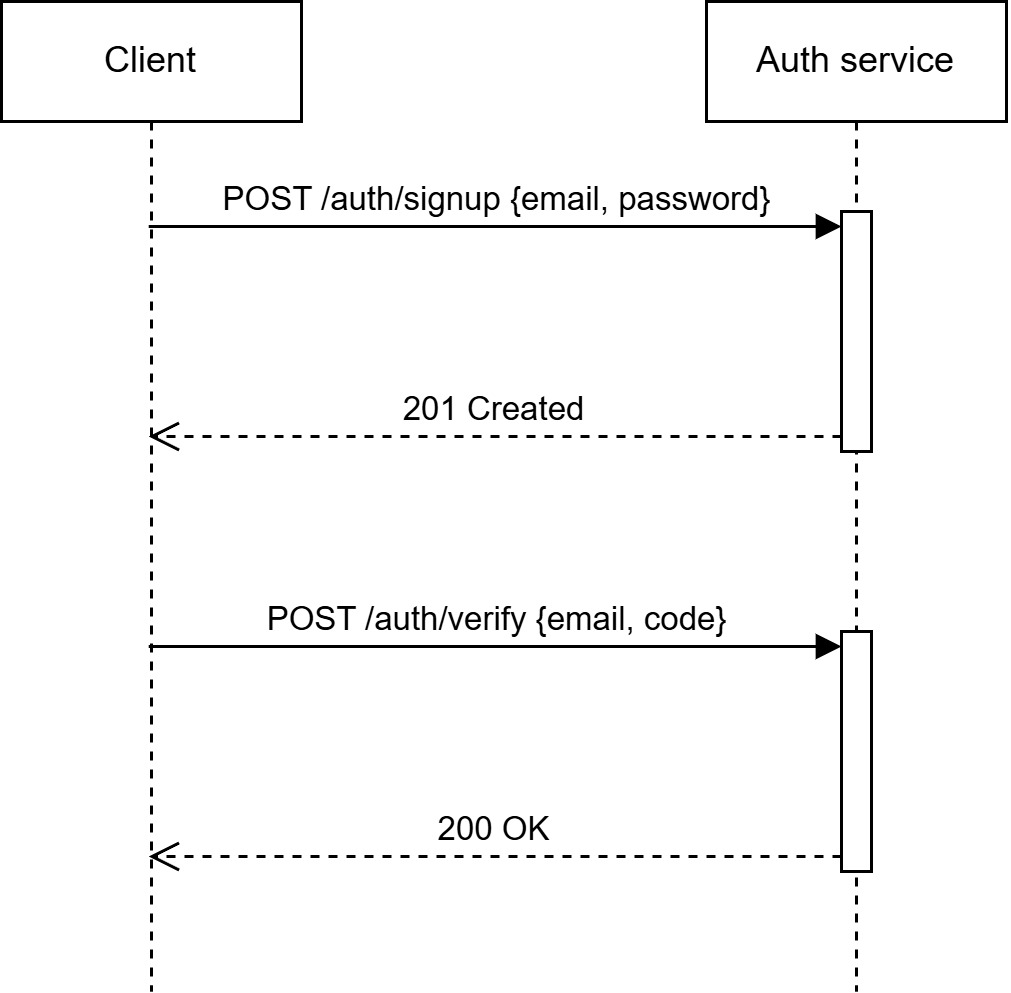
\includegraphics[width=0.55\textwidth]{img/09-technical-details/core-service/auth-service-case-1.jpg}
    \caption{Diagrama de secuencia del flujo de registro.}    \label{fig:auth-service-case-1}
\end{figure}

La verificación se realiza mediante \texttt{POST /auth/verify}, y el código se puede regenerar con 
\texttt{POST /auth/refresh}. La petición de verificación requiere enviar también el correo; se disponen de hasta tres 
intentos para verificar el código. Si se fallan los tres intentos, la cuenta queda en un estado inválido que impide volver 
a registrarse.
\vspace{0.25cm}

Posteriormente, se debe enviar una petición a \texttt{POST /auth/login}. Con esa petición se reciben los tokens de
acceso (\textit{access tokens}) para acceder a los \textit{endpoints} restringidos o que requieren autenticación. Los
tokens son \textit{JSON Web Tokens} (JWT), los cuales almacenan información relevante de la sesión, como el ID del
usuario y la fecha de expiración. La duración de estos tokens es de 1 día.
\vspace{0.25cm}

En caso de que la sesión venza, existe la posibilidad de regenerar el token mediante los tokens de refresco
(\textit{refresh tokens}), que tienen un vencimiento de 30 días. Para comprobar el estado de una sesión existe el
\textit{endpoint} \texttt{GET /auth/check-session}, que retorna el estado de la sesión; para regenerar los tokens se
utiliza \texttt{POST /auth/refresh-token}, que regenera el \textit{access token} y el \textit{refresh token}. 
\vspace{0.25cm}

Además, se actualiza en la tabla de usuarios la fecha de creación del último \textit{refresh token} para invalidar todos 
los tokens anteriores en caso de que el usuario haya sufrido un ataque de \textit{sniffing} de paquetes a través de un
"Man-in-the-Middle". De este modo, un usuario deberá volver a autenticarse solo si permanece 30 días seguidos inactivo.
\vspace{0.25cm}

El flujo de recuperación de contraseña consta de tres pasos. En primer lugar, el usuario envía una petición a
\texttt{POST /auth/password/forgot} con su dirección de correo electrónico. En caso de que el correo corresponda a una 
cuenta registrada, se genera un código OTP (\textit{One-Time Password}) y se envía al correo del usuario.
\vspace{0.25cm}

\begin{figure}[H]
    \centering
    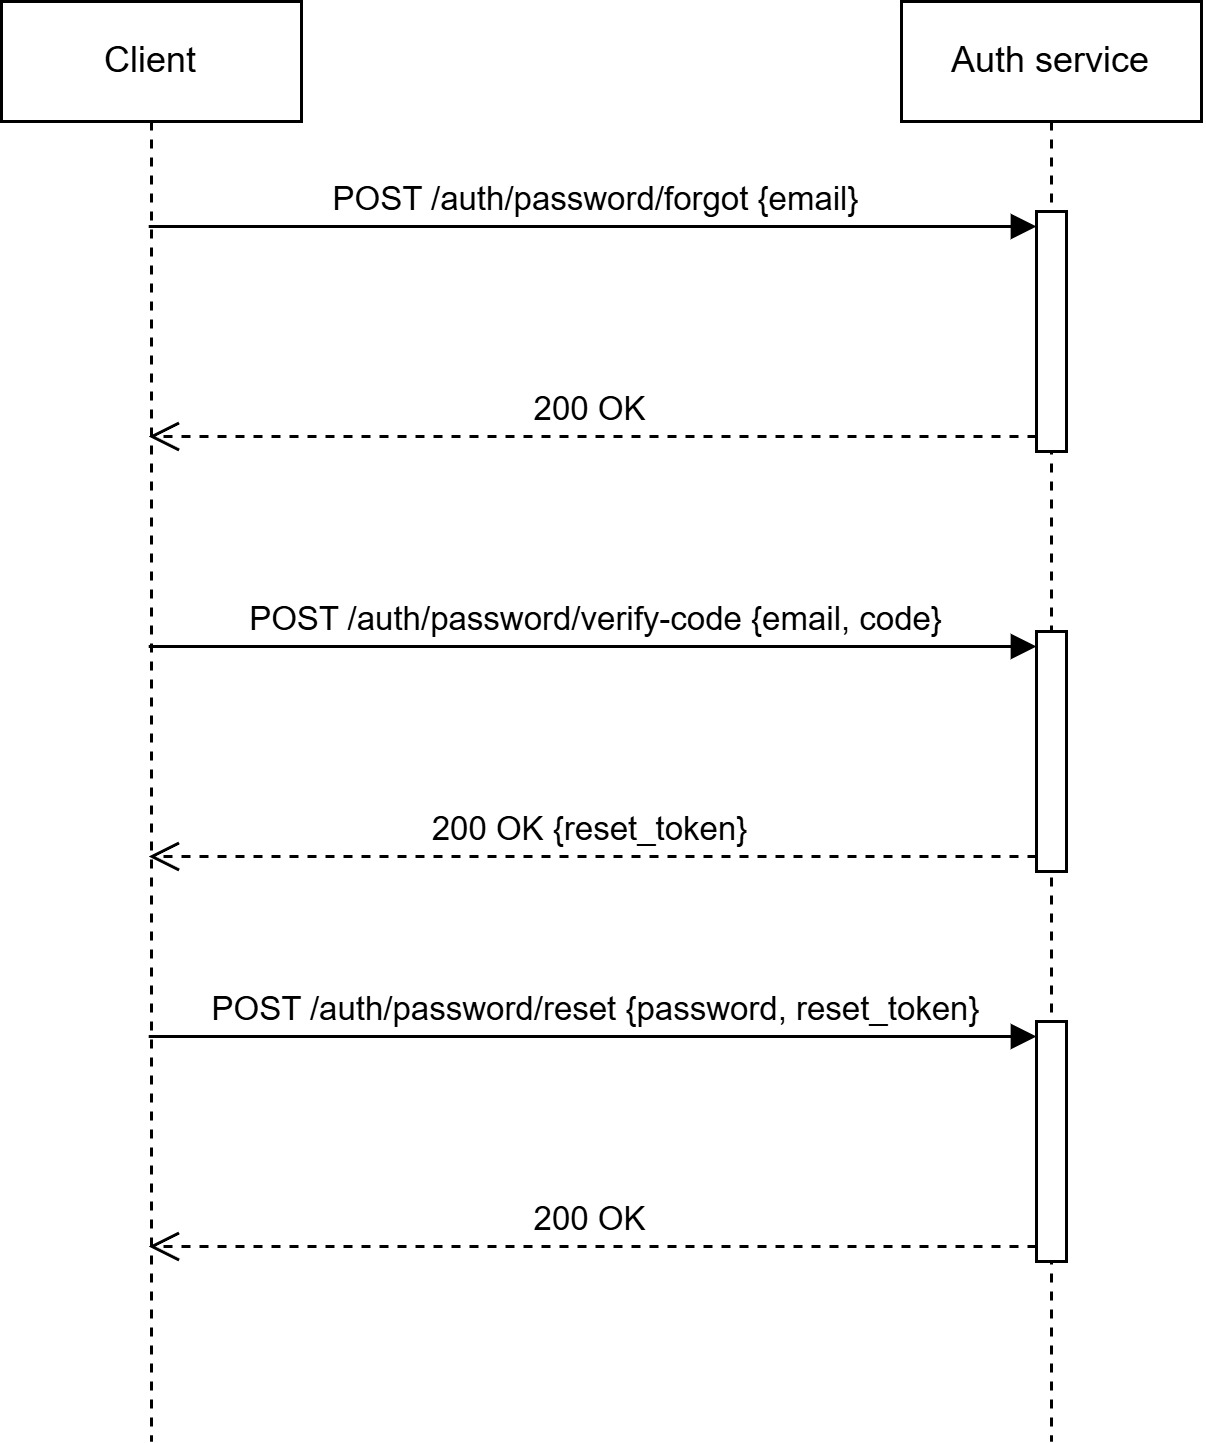
\includegraphics[width=0.65\textwidth]{img/09-technical-details/core-service/auth-service-case-2.jpg}
    \caption{Diagrama de secuencia del recuepero de contraseña.}    \label{fig:auth-service-case-2}
\end{figure}

A continuación, el usuario debe verificar el código recibido mediante el \textit{endpoint} \texttt{POST /auth/password/verify-code},
proporcionando su correo y el OTP. El sistema contempla distintas casuísticas de error, como código incorrecto,
código expirado o número máximo de intentos superado. Si el código es válido, se emite un token de restablecimiento
(\textit{reset token}) de corta duración. Y usuario completa el proceso enviando el \textit{reset token} junto con la 
nueva contraseña a \texttt{POST /auth/password/reset}. Si el token ha expirado o ya fue utilizado, el usuario deberá iniciar 
el flujo desde el principio.
\vspace{0.25cm}
